\section{Reducing the String Partitioning Problem to the MWPBM Problem}
\label{sec:reduction_to_mwpbm}

In the previous chapters, we modeled the task of partitioning trie nodes into $p$ chains as the String Partitioning Problem (see \cref{def:string_partitioning_problem}). We now demonstrate that this problem can be solved in polynomial time by reducing it to the MWPBM problem. This section will first detail the construction of a bipartite graph from an instance of the String Partitioning Problem. Then, we will prove that a minimum-weight perfect matching in this graph directly corresponds to an optimal solution for the partitioning problem. Let's start with an example.

\begin{example}[String Partitioning Problem]
    \label{ex:string_partitioning}
    Let $S = \text{AABACABB}$ be the input string and let $p=2$ be the desired number of subsequences. Our goal is to partition the characters of $S$ into two subsequences, $S_1$ and $S_2$, such that the total number of runs (\cref{def:run}) is minimized.

    Consider the following partition:
    \begin{itemize}
        \item $S_1$ is formed by taking the 1st, 2nd, 4th, and 6th characters of $S$: $\text{AAAA}$.
        \item $S_2$ is formed by the remaining characters (3rd, 5th, 7th, and 8th): $\text{BCBB}$.
    \end{itemize}
    
    The number of runs for each subsequence is:
    \begin{itemize}
        \item Runs($S_1$) = 1 (the run is "AAAA").
        \item Runs($S_2$) = 3 (the runs are "B", "C", "BB").
    \end{itemize}
    
    The total number of runs for this partition is $1 + 3 = 4$. An optimal solution to the String Partitioning Problem would be a partition that achieves the minimum possible total number of runs. In this case, 4 is indeed the optimal value.
\end{example}

\subsection{Bipartite Graph Construction}
Now, we will show how to construct a bipartite graph that allows us to solve the
String Partitioning problem.

\begin{definition}[Bipartite graph construction] \label{def:bip_construction}
    Let $A=a_1a_2\dots a_n$ be a string from an alphabet $\Sigma$ and let $p$ be the number of subsequences we want to partition $S$ in. 
    We can construct a weighted bipartite graph $G = (V,E,w)$ such that vertices are divided in two disjoint sets $V = V_1 \cup V_2$ in the following way:
    \begin{itemize}[leftmargin=25pt]
        \item $V_1$ contains $n+p$ nodes composed by $p$ source nodes $s_1,s_2,\dots,s_p$ (referred to collectively as $\sourceset$) followed by the $n$ characters $a_1,a_2,\dots,a_n$ (referred to collectively as $\treeset{1}$) of $A$. The nodes in $V_1$ follow a strict ordering $s_1 \prec s_2 \prec \dots \prec s_p \prec a_1 \prec a_2 \prec \dots \prec a_n$.
        \item $V_2$ contains $n+p$ nodes composed by the $n$ characters $a_1,a_2,\dots,a_n$ (referred to collectively as $\treeset{2}$) of $A$ followed by $p$ destination nodes $d_1,d_2,\dots,d_p$ (referred to collectively as $\destset$). The nodes in $V_2$ follow a strict ordering $a_1 \prec a_2 \prec \dots \prec a_n \prec d_1 \prec d_2 \prec \dots \prec d_p$.
    \end{itemize}
    Then the edges of the graph $G$ are constructed in the following way:
    \begin{itemize}[leftmargin=25pt]
        \item \textbf{Source Edges:} For each source node $s \in \sourceset$ and each node $v_j \in \treeset{2}$, an edge $(s, v_j)$ is created with weight $w(s, v_j) = 1$. These edges represent the start of a new subsequence.

        \item \textbf{Internal nodes Edges:} For each pair of indices $i, j$ such that $1 \le i < j \le n$, an edge is created between $u_i \in \treeset{1}$ and $v_j \in \treeset{2}$. The weight of this edge, $w(u_i, v_j)$, is 0 if the characters $A[i]$ and $A[j]$ are the same, and 1 otherwise. Formally:
        \[ w(u_i, v_j) = 
            \begin{cases} 
                0 & \text{if } A[i] = A[j] \\
                1 & \text{if } A[i] \neq A[j] 
            \end{cases}
        \]
        This weight represents the cost of adding character $A[j]$ after $A[i]$ in a subsequence, where a cost of 1 is incurred if a new run is started.

        \item \textbf{Destination Edges:} For each node $u_i \in \treeset{1}$ and each destination node $d \in \destset$, an edge $(u_i, d)$ is created with weight $w(u_i, d) = 1$. These edges represent the end of a subsequence.
    \end{itemize}
\end{definition}

\begin{example}[Vertices] \label{ex:reduction_vertices}
    Let's apply the reduction to the string $S = \text{ABCDDCBDDDD}$ from our running example (\cref{ex:string_example}), with a target of $p=2$ subsequences. Following the construction rules, we build a bipartite graph. The vertices of this graph are structured as shown in \cref{fig:bipartite_structure}.
    
    % Second figure - Bipartite graph structure
    \begin{figure}[H]
        \centering
        \tikzset{main/.style = {draw, circle, thick, minimum size=8mm, inner sep=0pt}}
        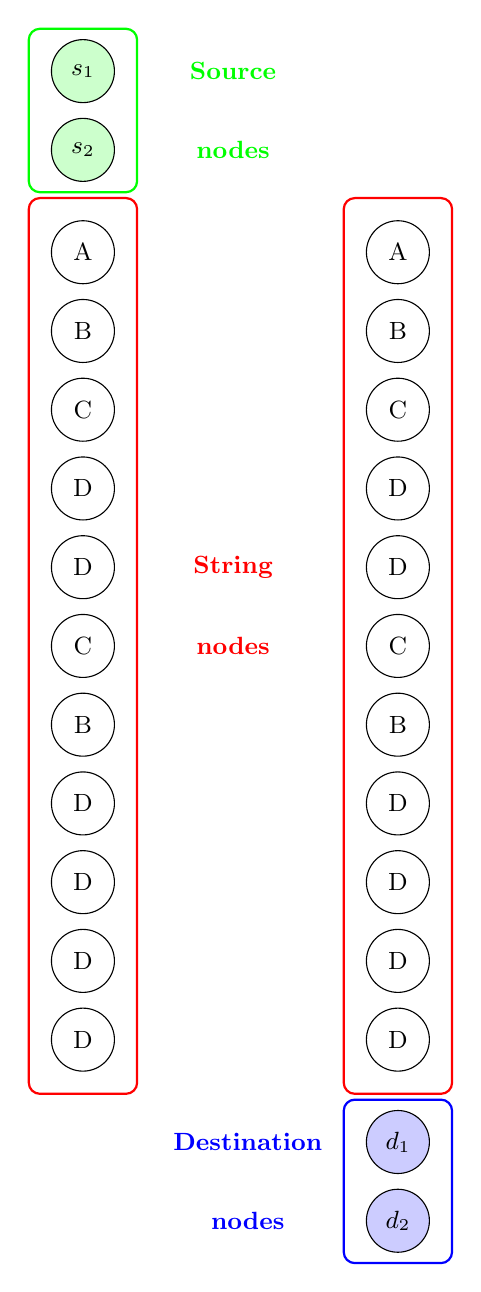
\begin{tikzpicture}[node distance=10mm]
            % Define node styles
            \tikzstyle{main} = [circle, draw, minimum size=0.8cm, font=\small]
            \tikzstyle{source} = [circle, draw, minimum size=0.8cm, font=\small, fill=green!20]
            \tikzstyle{dest} = [circle, draw, minimum size=0.8cm, font=\small, fill=blue!20]
            
            % Source nodes (left column, green background)
            \node[source] (s1) {$s_1$};
            \node[source] (s2) [below of=s1] {$s_2$};
            
            % Tree nodes (left column, red border)
            \node[main] (t1) [below of=s2, yshift=-0.3cm] {A};
            \node[main] (t2) [below of=t1] {B};
            \node[main] (t3) [below of=t2] {C};
            \node[main] (t4) [below of=t3] {D};
            \node[main] (t5) [below of=t4] {D};
            \node[main] (t6) [below of=t5] {C};
            \node[main] (t7) [below of=t6] {B};
            \node[main] (t8) [below of=t7] {D};
            \node[main] (t9) [below of=t8] {D};
            \node[main] (t10) [below of=t9] {D};
            \node[main] (t11) [below of=t10] {D};
            
            % Tree nodes (right column, red border)
            \node[main] (r1) [right of=t1, xshift=3cm] {A};
            \node[main] (r2) [below of=r1] {B};
            \node[main] (r3) [below of=r2] {C};
            \node[main] (r4) [below of=r3] {D};
            \node[main] (r5) [below of=r4] {D};
            \node[main] (r6) [below of=r5] {C};
            \node[main] (r7) [below of=r6] {B};
            \node[main] (r8) [below of=r7] {D};
            \node[main] (r9) [below of=r8] {D};
            \node[main] (r10) [below of=r9] {D};
            \node[main] (r11) [below of=r10] {D};
            
            % Destination nodes (right column, blue background)
            \node[dest] (d1) [below of=r11, yshift=-0.3cm] {$d_1$};
            \node[dest] (d2) [below of=d1] {$d_2$};
            
            % Draw colored rectangles around groups
            % Green rectangle for source nodes
            \draw[green, thick, rounded corners] ([xshift=-0.4cm,yshift=0.25cm]s1.north west) rectangle ([xshift=0.4cm,yshift=-0.25cm]s2.south east);
            
            % Red rectangle for left tree nodes
            \draw[red, thick, rounded corners] ([xshift=-0.4cm,yshift=0.4cm]t1.north west) rectangle ([xshift=0.4cm,yshift=-0.4cm]t11.south east);
            
            % Red rectangle for right tree nodes
            \draw[red, thick, rounded corners] ([xshift=-0.4cm,yshift=0.4cm]r1.north west) rectangle ([xshift=0.4cm,yshift=-0.4cm]r11.south east);
            
            % Blue rectangle for destination nodes
            \draw[blue, thick, rounded corners] ([xshift=-0.4cm,yshift=0.25cm]d1.north west) rectangle ([xshift=0.4cm,yshift=-0.25cm]d2.south east);
            
            % Add labels
            \node[green!100, font=\small\bfseries] at ([xshift=1.5cm]s1.east) {Source};
            \node[green!100, font=\small\bfseries] at ([xshift=1.5cm]s2.east) {nodes};
            
            \node[red, font=\small\bfseries] at ([xshift=1.5cm]t5.east) {String};
            \node[red, font=\small\bfseries] at ([xshift=1.5cm]t6.east) {nodes};
            
            \node[blue, font=\small\bfseries] at ([xshift=-1.5cm]d1.west) {Destination};
            \node[blue, font=\small\bfseries] at ([xshift=-1.5cm]d2.west) {nodes};
            
            % Add "Corresponding tree node" label with arrow
            % \draw[<->, thick] (t1.east) -- (r1.west);
            % \node[font=\small] at ([xshift=0cm,yshift=-0.25cm]$(t1)!0.5!(r1)$) {Corresponding};
            % \node[font=\small] at ([xshift=0cm,yshift=-0.7cm]$(t1)!0.5!(r1)$) {tree node};
            
        \end{tikzpicture}
        \caption{Bipartite graph vertices structure for string $S = \text{ABCDDCBDDDD}$ with $p=2$. The nodes are ordered from top to bottom.}
        \label{fig:bipartite_structure}
    \end{figure}
\end{example}

\begin{example}[Edges]
    Let's see a small example for each case of \cref{def:bip_construction}. Consider $p=2$. In \cref{fig:reduction_small_examples}-(a), there is an example for the sources' edges. As stated before, each source is connected with weight $1$ to all nodes in $\treeset{2}$.

    In \cref{fig:reduction_small_examples}-(b), we illustrate the edges from $\treeset{1}$ to $\treeset{2}$. These edges model the cost of appending a character to a subsequence. An edge from $u_i$ to $v_j$ (for $j>i$) has weight 1 if $S[i] \neq S[j]$ (starting a new run) and weight 0 if $S[i] = S[j]$ (extending an existing run). For instance, the node for the first 'A' connects to the nodes for 'B' and 'C' with weight 1, but connects to the node for 'A' with weight 0.

    Lastly, \cref{fig:reduction_small_examples}-(c) shows the destination edges. These edges terminate a subsequence. An edge from any node $u_i \in \treeset{1}$ to any destination node $d_k \in \destset$ has a weight of 0, ensuring that ending a chain does not increase the run count. For example, if the node for 'B' is the last element of a subsequence, it is matched with a destination node, and this edge $(u_B, d_k)$ contributes 0 to the total weight.

    \begin{figure}[H]
        \centering
        \tikzset{main/.style = {draw, circle, thick, minimum size=8mm, inner sep=0pt}}
        \begin{subfigure}[b]{0.3\textwidth}
            \centering
            \begin{tikzpicture}[node distance=10mm, auto=center]
                \tikzstyle{main} = [circle, draw, minimum size=0.8cm, font=\small]
                \tikzstyle{source} = [circle, draw, minimum size=0.8cm, font=\small, fill=green!20]
                \tikzstyle{dest} = [circle, draw, minimum size=0.8cm, font=\small, fill=blue!20]
                
                % Left column (sources)
                \node[source] (1s) {$s_1$};
                \node[source] (2s) [below of=1s] {$s_2$};
                \node[main] (3s) [below of=2s] {A};
                \node[right=0cm of 3s] {$\cdots$};
                \node[main] (4s) [below of=3s] {A};
                \node[right=0cm of 4s] {$\cdots$};
                \node[main] (5s) [below of=4s] {B};
                \node[right=0cm of 5s] {$\cdots$};
                \node (dots_s) [below of=5s] {\vdots}; % Vertical dots

                % Right column (destinations)
                \node[main] (1d) [right=2.5cm of 3s] {A};
                \node[main] (2d) [below of=1d] {A};
                \node[left=0cm of 2d] {$\cdots$};
                \node[main] (3d) [below of=2d] {B};
                \node[left=0cm of 3d] {$\cdots$};
                \node (dots_d) [below of=3d] {\vdots}; % Vertical dots

                % Arrows
                \draw[red, ->] (1s) -- (1d);
                \draw[red, ->] (1s) -- (2d);
                \draw[red, ->] (1s) -- (3d);
                \draw[red, ->] (2s) -- (1d);
                \draw[red, ->] (2s) -- (2d);
                \draw[red, ->] (2s) -- (3d);
            \end{tikzpicture}
            \caption{}
            \label{fig:sub1}
        \end{subfigure}
        \hfill % Space between subfigures
        \tikzset{main/.style = {draw, circle, thick, minimum size=8mm, inner sep=0pt}}
        \begin{subfigure}[b]{0.3\textwidth}
            \centering
            \begin{tikzpicture}[node distance=10mm, auto=center]
                \tikzstyle{main} = [circle, draw, minimum size=0.8cm, font=\small]
                \tikzstyle{source} = [circle, draw, minimum size=0.8cm, font=\small, fill=green!20]
                \tikzstyle{dest} = [circle, draw, minimum size=0.8cm, font=\small, fill=blue!20]

                % Left column (tree nodes)
                \node (dots_s_top) {\vdots};
                \node[main] (3s) [below of=dots_s_top] {A};
                \node[main] (4s) [below of=3s] {B};
                \node[right=0cm of 4s] {$\cdots$};
                \node[main] (5s) [below of=4s] {A};
                \node[right=0cm of 5s] {$\cdots$};
                \node[main] (6s) [below of=5s] {C};
                \node[right=0cm of 6s] {$\cdots$};
                \node (dots_s_bottom) [below of=6s] {\vdots};

                % Right column (destinations)
                \node (dots_d_top) [right=2.5cm of dots_s_top] {\vdots};
                \node[main] (1d) [below of=dots_d_top] {A};
                \node[left=0cm of 1d] {$\cdots$};
                \node[main] (2d) [below of=1d] {B};
                \node[left=0cm of 2d] {$\cdots$};
                \node[main] (3d) [below of=2d] {A};
                \node[left=0cm of 3d] {$\cdots$};
                \node[main] (4d) [below of=3d] {C};
                \node[left=0cm of 4d] {$\cdots$};
                \node (dots_d_bottom) [below of=4d] {\vdots};

                % Arrows
                \draw[red, ->] (3s) -- (2d);
                \draw[red, ->] (3s) -- (4d);
                \draw[green, ->] (3s) -- (3d);
            \end{tikzpicture}
            \caption{}
            \label{fig:sub2}
        \end{subfigure}
        \hfill % Space between subfigures
        \tikzset{main/.style = {draw, circle, thick, minimum size=8mm, inner sep=0pt}}
        \begin{subfigure}[b]{0.3\textwidth}
            \centering
            \begin{tikzpicture}[node distance=10mm, auto=center]
                \tikzstyle{main} = [circle, draw, minimum size=0.8cm, font=\small]
                \tikzstyle{source} = [circle, draw, minimum size=0.8cm, font=\small, fill=green!20]
                \tikzstyle{dest} = [circle, draw, minimum size=0.8cm, font=\small, fill=blue!20]

                % Left column (original destinations)
                \node (dots_s_top) {\vdots};
                \node[main] (7s) [below of=dots_s_top] {A};
                \node[main] (9s) [below of=7s] {B};

                % Right column (bipartite graph destinations)
                \node (dots_d_top) [right=2.5cm of dots_s_top] {\vdots};
                \node[main] (5d) [below of=dots_d_top] {A};
                \node[left=0cm of 5d] {$\cdots$};
                \node[main] (6d) [below of=5d] {B};
                \node[left=0cm of 6d] {$\cdots$};
                \node[dest] (8d) [below of=6d] {$d_1$};
                \node[left=0cm of 8d] {$\cdots$};
                \node[dest] (9d) [below of=8d] {$d_2$};
                \node[left=0cm of 9d] {$\cdots$};

                % Arrows
                \draw[red, ->] (7s) -- (6d);
                \draw[green, ->] (7s) -- (8d);
                \draw[green, ->] (7s) -- (9d);
                \draw[green, ->] (9s) -- (8d);
                \draw[green, ->] (9s) -- (9d);
            \end{tikzpicture}
            \caption{}
            \label{fig:sub3}
        \end{subfigure}

        \caption[Examples of reduction to a bipartite graph]{Examples of the connection construction in the bipartite graph for $p=2$, showing the cases for source nodes $\sourceset$ (a), internal nodes $\treeset{1}$ and $\treeset{2}$ (b), and destination nodes $\destset$ (c). Red arrows indicate edges with weight 1, while green arrows indicate edges with weight 0.}
        \label{fig:reduction_small_examples}
    \end{figure}
\end{example}

let now state the following theorem regarding the number of edges in the bipartite graph resulting from \cref{def:bip_construction}. This theorem is essential for understanding the complexity of the final algorithm employed to solve the MWPBM problem and so, the String Partitioning problem.

\begin{theorem}[Bipartite graph properties] \label{thm:bip_graph_properties}
    The bipartite graph $G$ constructed as stated in \cref{def:bip_construction} has $2n + 2p$ nodes and $2np + \frac{n(n-1)}{2}$ edges.
\end{theorem}

\begin{proof}
    The total number of edges in the graph $G$ is the sum of the edges from the three categories defined in the construction:
    \begin{itemize}[leftmargin=25pt]
        \item \textbf{Source Edges:} There are $p$ source nodes in $\sourceset$ and $n$ tree nodes in $\treeset{2}$. Each source node connects to every node in $\treeset{2}$, resulting in $p \times n = np$ edges.

        \item \textbf{Destination Edges:} There are $n$ tree nodes in $\treeset{1}$ and $p$ destination nodes in $\destset$. Each node in $\treeset{1}$ connects to every node in $\destset$, resulting in $n \times p = np$ edges.

        \item \textbf{Internal nodes Edges:} For each node $u_i \in \treeset{1}$, edges are created to all nodes $v_j \in \treeset{2}$ where $j > i$. The number of such edges is $\sum_{i=1}^{n-1} (i) = \frac{n(n-1)}{2}$.
    \end{itemize}

    Summing these up, the total number of edges is $2np + \frac{n(n-1)}{2}$.
\end{proof}

\subsection{Proof}
In this section, we will prove that a minimum-weight perfect matching in a bipartite graph constructed as stated in \cref{def:bip_construction} directly corresponds to an optimal solution for the String Partitioning problem. 

Let's start by defining the concept of valid partition:
\begin{definition}[Valid Partition]
    \label{def:valid_partition}
    A partition of a string $S$ into $p$ subsequences, denoted $\Pi = \{S_1, S_2, \dots, S_p\}$, is \textbf{valid} if it satisfies two conditions:
    \begin{enumerate}[leftmargin=25pt]
        \item \textbf{Character Conservation:} The multiset of characters in $S$ is the disjoint union of the multisets of characters in each subsequence $S_i$. This ensures every character from $S$ is used exactly once.
        \item \textbf{Order Preservation:} For any subsequence $S_k \in \Pi$, if $S_k$ contains characters corresponding to $S[i]$ and $S[j]$ from the original string with $i < j$, then the character from $S[i]$ must appear before the character from $S[j]$ in $S_k$.
    \end{enumerate}
\end{definition}

We also define $runs(S)$ as the number of runs in the string $S$.

\begin{lemma} \label{lemma:optimal_cost}
    Let $\Sigma_S \subseteq \Sigma$ be the set of unique characters that appear in the string $S$. The cost of the optimal solution of an instance $\mathcal{I}=(S,p)$ of the String Partitioning Problem is always greater than or equal to $|\Sigma_S|$, for any $p$.
\end{lemma}

\begin{proof}
    Let $\Pi = \{S_1, S_2, \dots, S_p\}$ be any valid partition of the string $S$ into $p$ subsequences. The cost of this partition is the total number of runs, given by $\sum_{i=1}^{p} \text{runs}(S_i)$.

    For any character $c \in \Sigma_S$, there must be at least one occurrence of $c$ in $S$. This occurrence must be placed in at least one of the subsequences, say $S_j$. The first occurrence of character $c$ in any subsequence $S_j$ will start a new run. For each distinct character in $\Sigma_S$, its occurrences must form at least one run in the partition. If a character appears in multiple subsequences, it will contribute at least one run for each subsequence it is in. If it appears only in one subsequence, it will contribute at least one run to that subsequence.

    Therefore, every unique character $c \in \Sigma_S$ must contribute at least one run to the total cost. Summing over all unique characters, the total number of runs must be at least $|\Sigma_S|$.
\end{proof}

\begin{claim} \label{claim:p_greater_than_alphabet_size}
    For the String Partitioning Problem, the optimal cost for an instance $\mathcal{I}=(S, p)$ where $p > |\Sigma_S|$ is not lower than the optimal cost for the instance $\mathcal{M}=(S, |\Sigma_S|)$, where $\Sigma_S$ is the set of unique characters in $S$.
\end{claim}

\begin{proof}
    The proof builds upon \cref{lemma:optimal_cost}. If we use a number of chains $p > |\Sigma_S|$, we would have at least $p - |\Sigma_S|$ empty chains, since there are only $|\Sigma_S|$ non-empty equivalence classes of nodes to partition. As the minimum cost for any chain is 1, these empty chains contribute to the total cost. An optimal arrangement would involve $|\Sigma_S|$ chains, each containing nodes from a single equivalence class, costing $|\Sigma_S|$, and $p - |\Sigma_S|$ empty chains, each costing 1. The total cost would be $|\Sigma_S| + (p - |\Sigma_S|) = p$. Since $p > |\Sigma_S|$, this cost is greater than the optimal cost of $|\Sigma_S|$ achievable with $p = |\Sigma_S|$ chains. Therefore, any solution with $p > |\Sigma_S|$ is suboptimal.
\end{proof}

Therefore, we will only consider instances of the problem where $p < |\Sigma_S|$, as they do not present a trivial solution.

Let $r:\mathcal{I}_{String Partitioning} \rightarrow \mathcal{M}_{MWPBM}$ be the reduction function that maps an instance $\mathcal{I}=(S, p)$ of the String Partitioning Problem to an instance $\mathcal{M}=(G)$ of the MWPBM Problem, where $G$ is the bipartite graph constructed as stated in \cref{def:bip_construction}.
\begin{claim} \label{lemma:greater_nodes}
    Let $\mathcal{I}=(S, p)$ be an instance of the String Partitioning Problem. In any perfect matching on $r(\mathcal{I})$, a node $u_i \in \treeset{1}$ can only be matched with a node $v_j \in \treeset{2}$ if $j > i$.
\end{claim}

\begin{proof}
    This property is a direct consequence of the definition of internal edges in the graph construction. Edges between the sets $\treeset{1}$ and $\treeset{2}$ are explicitly defined only for pairs of nodes $(u_i, v_j)$ where the index $j$ is strictly greater than $i$. No edges are created for any case where $j \le i$.

    Since a matching is a subset of the graph's edges, it is impossible for a node $u_i$ to be matched with a node $v_j$ with an equal or smaller index. This structural constraint is fundamental to ensuring that the subsequences in the partition respect the original order of characters in the string $S$ leading to a valid partition of the string.
\end{proof}

\begin{lemma} \label{lemma:matching_existence}
    Let $\mathcal{I}=(S, p)$ be an instance of the String Partitioning Problem. There always exists a perfect matching on $r(\mathcal{I})$.
\end{lemma}

\begin{proof}
    Let $G$ be the bipartite graph of the MWPBM instance $r(\mathcal{I})$. The proof comes from the construction of the bipartite graph $G$ and from \cref{thm:halls_marriage_theorem}. We are going to prove that $G$ satisfies Hall's condition (see \cref{thm:halls_marriage_theorem}) and so, since by construction $|V_1| = |V_2|$, a perfect matching for $G$ exists.

    To verify Hall's condition, we need to prove that for any subset $W \subseteq V_1$ we have that $|N(W)| \geq |W|$, where $N(W)$ is the neighborhood of $W$ (\cref{def:neighborhood}). We have the following cases:
    \begin{itemize}[leftmargin=25pt]
        \item If $W \subseteq \sourceset$: Let $|W| = k$, where $1 \le k \le p$. By construction, every source node in $\sourceset$ is connected to every node in $\treeset{2}$. Therefore, the neighborhood of any non-empty subset $W \subseteq \sourceset$ is the entire set $\treeset{2}$, so $N(W) = \treeset{2}$. The size of the neighborhood is $|N(W)| = |\treeset{2}| = n$. We need to show that $n \ge k$. From the problem definition, we can assume $p \le n$, since having more partitions than characters offers no advantage (\cref{claim:p_greater_than_alphabet_size}). As $W$ is a subset of $\sourceset$, we have $k \le p$. Therefore, $k \le p \le n$, which confirms that $|N(W)| \ge |W|$. 
        
        \item If $W \subseteq \treeset{1}$, Let $|W| = k$. Let the indices of the nodes in $W$ be $\{i_1, i_2, \dots, i_k\}$, sorted such that $i_1 < i_2 < \dots < i_k$.
        
        By the construction of the graph, every node $u_i \in \treeset{1}$ is connected to every destination node in $\destset$. Therefore, the entire set $\destset$ is part of the neighborhood of $W$, so $\destset \subseteq N(W)$. This contributes $p$ nodes to the neighborhood.

        Additionally, each node $u_{i_r} \in W$ is connected to all nodes $v_j \in \treeset{2}$ where $j > i_r$. The union of these neighbors in $\treeset{2}$ is $\bigcup_{r=1}^{k} \{v_j \mid j > i_r\} = \{v_j \mid j > i_1\}$, since for any $r > 1$, the set $\{v_j \mid j > i_r\}$ is a subset of $\{v_j \mid j > i_1\}$. The size of this set of neighbors in $\treeset{2}$ is $n - i_1$.
        
        Combining these, the total size of the neighborhood is $|N(W)| = |\{v_j \mid j > i_1\} \cup \destset| = (n - i_1) + p$.
        
        We need to prove that $|N(W)| \ge |W|$, which means we must show $n - i_1 + p \ge k$.
        
        Since the $k$ indices in $W$ are distinct and sorted, we know that $i_k \ge i_1 + k - 1$. As $i_k \le n$, it follows that $i_1 + k - 1 \le n$, which can be rearranged to $k \le n - i_1 + 1$.
        
        Since $p \ge 2$ (as there is at least two partitions), we have $n - i_1 + p \ge n - i_1 + 2$.
        Combining these inequalities, we get $|N(W)| = n - i_1 + p \ge n - i_1 + 2 \ge k$.
        
        Thus, $|N(W)| \ge |W|$ holds for this case. 
        
        \item If $W=W_S \cup W_U$, where $W_S \subseteq \sourceset, W_U \subseteq \treeset{1}$. By construction:
        \begin{itemize}
            \item Since $W_S$ is a non-empty subset of $\sourceset$, every node in $W_S$ is connected to every node in $\treeset{2}$. Thus, the neighborhood of $W_S$ is the entire set $\treeset{2}$, so $N(W_S) = \treeset{2}$.
            \item Since $W_U$ is a non-empty subset of $\treeset{1}$, every node in $W_U$ is connected to every node in $\destset$. Thus, the neighborhood of $W_U$ includes the entire set $\destset$, so $N(W_U) \supseteq \destset$.
        \end{itemize}
        
        Combining these, the neighborhood of the mixed set $W$ contains both $\treeset{2}$ and $\destset$:
        $N(W) = N(W_S) \cup N(W_U) = \treeset{2} \cup \destset$.
        
        Since the entire right side of the bipartition is $V_2 = \treeset{2} \cup \destset$, this means the neighborhood of $W$ is the entire set $V_2$. Thus, $|N(W)| \ge |W|$ holds for this case. 
    \end{itemize}
    Since Hall's condition is satisfied for all possible non-empty subsets of $V_1$, a perfect matching always exists in the graph $G$.
\end{proof}

Before proving the main theorem, we need to define how to retrieve an optimal partitions for an instance of the String Partitioning Problem $\mathcal{I}=(S, p)$ from an optimal perfect matching in $r(\mathcal{I})$.

\begin{definition}[Partition decomposition] \label{def:partition_decomposition}
    Given an instance of the String Partitioning Problem $\mathcal{I}=(S, p)$ and an optimal perfect matching $M$ in the bipartite graph $G$ of $r(\mathcal{I})$, a \textbf{partition decomposition} of $M$ is a way to partition the nodes of $G$ into $p$ non-empty subsets, where each subset represents a path from a source to a destination, thus, leading to a partition of $S$. The partition decomposition proceed as follows:

    Since $M$ is a perfect matching, each source node $s_k \in \sourceset$ begins exactly one path. This path is a sequence of characters from $S$ determined by following the edges of $M$. A path starting from $s_k$ corresponds to a sequence of indices $(j_1, j_2, \dots, j_m)$ such that:
    \begin{enumerate}[leftmargin=25pt]
        \item The first edge is $(s_k, v_{j_1}) \in M$.
        \item Then, $(u_{j_i}, v_{j_{i+1}}) \in M \text{ } \forall \text{ } i=1,\dots,m-1$.
        \item The final edge in the path is $(u_{j_m}, d_q) \in M$ for some destination node $d_q$.
    \end{enumerate}
    The subsequence $S_k$ is then constructed from the characters at these indices: $S_k = S[j_1]S[j_2]\dots S[j_m]$. This process uniquely defines a valid partition of $S$ into $p$ subsequences.
\end{definition}

\begin{example}
    Consider the example in \cref{fig:example_bipartite_read}, which shows a perfect matching for the instance $r(\mathcal{I})$ with $\mathcal{I}=(S=\text{AAB}, p=2)$. The solid arrows represent the edges of the matching $M$. The dashed arrows are a visual aid showing the correspondence between a character's representation in $\treeset{2}$ (on the right) and its representation in $\treeset{1}$ (on the left), which is essential for tracing the paths.

    Applying the partition decomposition procedure (\cref{def:partition_decomposition}), we extract two subsequences:

    \begin{itemize}
        \item \textbf{Subsequence 1 (red):}
        \begin{enumerate}
            \item Start at source $s_1$. The matching edge is $(s_1, v_1)$, where $v_1$ corresponds to the first character, $S[1] = \text{'A'}$. The subsequence is now "A".
            \item Following the conceptual link to $u_1$, we find the matching edge $(u_1, v_2)$, where $v_2$ corresponds to the second character, $S[2] = \text{'A'}$. The subsequence is now "AA".
            \item Following the link to $u_2$, we find the matching edge $(u_2, d_1)$. Since $d_1$ is a destination node, the path terminates.
            \item The final subsequence is $S_1 = \text{"AA"}$.
        \end{enumerate}

        \item \textbf{Subsequence 2 (blue):}
        \begin{enumerate}
            \item Start at source $s_2$. The matching edge is $(s_2, v_3)$, where $v_3$ corresponds to the third character, $S[3] = \text{'B'}$. The subsequence is "B".
            \item Following the link to $u_3$, we find the matching edge $(u_3, d_2)$. Since $d_2$ is a destination, the path terminates.
            \item The final subsequence is $S_2 = \text{"B"}$.
        \end{enumerate}
    \end{itemize}
    This example illustrates how the partition decomposition procedure correctly reconstructs the subsequences from the perfect matching, yielding the partition $\Pi = \{\text{"AA"}, \text{"B"}\}$.
    \begin{figure}[H]
        \centering
        \tikzset{main/.style = {draw, circle, thick, minimum size=8mm, inner sep=0pt}}
        \begin{tikzpicture}[node distance=10mm, auto=center]
            \tikzstyle{main} = [circle, draw, minimum size=0.8cm, font=\small]
            \tikzstyle{source} = [circle, draw, minimum size=0.8cm, font=\small, fill=green!20]
            \tikzstyle{dest} = [circle, draw, minimum size=0.8cm, font=\small, fill=blue!20]

            % Left column (original destinations)
            \node[source] (1s) {$s_1$};
            \node[source] (2s) [below of=1s] {$s_2$};
            \node[main] (7s) [below of=2s] {A};
            \node[main] (8s) [below of=7s] {A};
            \node[main] (9s) [below of=8s] {B};

            % Right column (bipartite graph destinations)
            \node[main] (5d) [right=2.5cm of 7s] {A};
            \node[main] (7d) [below of=5d] {A};
            \node[main] (6d) [below of=7d] {B};
            \node[dest] (8d) [below of=6d] {$d_1$};
            \node[dest] (9d) [below of=8d] {$d_2$};

            % Arrows
            \draw[red, ->] (1s) -- (5d);
            \draw[red, ->] (7s) -- (7d);
            \draw[red, ->] (8s) -- (8d);
            \draw[red, dashed, ->] (5d) -- (7s);
            \draw[red, dashed, ->] (7d) -- (8s);

            \draw[blue, ->] (2s) -- (6d);
            \draw[blue, ->] (9s) -- (9d);
            \draw[blue, dashed, ->] (6d) -- (9s);
        \end{tikzpicture}
        \caption{An example of a perfect matching (solid lines) in the constructed bipartite graph. The matching defines a partition into two paths (red and blue), which are traced by following the solid and dashed arrows.}
        \label{fig:example_bipartite_read}
    \end{figure}
\end{example}

Now we introduce the main theorem for the reduction.

\begin{theorem}
    Let $\mathcal{I}=(S,p)$ be an instance of the String Partition problem with $S=a_1a_2\dots a_n$. An optimal solution of $r(\mathcal{I})$ can be used to compute an optimal solution of $\mathcal{I}$ in time $O(2np + \frac{n(n-1)}{2})$.
\end{theorem}

\begin{proof}
    Let $\mathcal{I} = (S, p)$ be an instance of the String Partitioning problem. We assume $p \leq |\Sigma_S|$ where $\Sigma_S$ is the set of unique characters in $S$, per \cref{claim:p_greater_than_alphabet_size}. Let $G$ be the bipartite graph of instance $r(\mathcal{I})$. We will demonstrate a bijection between the set of valid partitions of $S$ (see \cref{def:valid_partition}) and the set of perfect matchings in $G$, such that the cost of a partition equals the weight of its corresponding perfect matching.

    First, we establish the existence of a perfect matching. By construction, the graph $G$ is bipartite with partitions $V_1$ and $V_2$ such that $|V_1| = |V_2| = t+p$. \cref{lemma:matching_existence} ensures that a perfect matching exists in $G$.

    Let $\Pi = \{S_1, \dots, S_p\}$ be a valid partition of $S$. We construct a perfect matching $M_\Pi$ by converting each subsequence $S_k \in \Pi$ into a path in $G$. Let the ordered indices of $S_k$ be $i_{k,1} < i_{k,2} < \dots < i_{k,l_k}$. The corresponding path in $G$ is formed by the following edges:
    \begin{itemize}[leftmargin=25pt]
        \item A \textbf{start edge} $(s_k, v_{i_{k,1}})$. This edge exists because all source nodes are connected to all nodes in $\treeset{2}$.
        \item A set of \textbf{middle edges} $(u_{i_{k,j}}, v_{i_{k,j+1}})$ for $j=1, \dots, l_k-1$. These edges exist because the order preservation property of a valid partition ensures $i_{k,j} < i_{k,j+1}$, and our graph construction connects $u_i \in \treeset{1}$ to $v_j \in \treeset{2}$ for all $i < j$.
        \item An \textbf{end edge} $(u_{i_{k,l_k}}, d_k)$. This edge exists because all nodes in $\treeset{1}$ are connected to all destination nodes.
    \end{itemize}
    Since every character of $S$ belongs to exactly one subsequence, this process uses every node in $\treeset{1}$ and $\treeset{2}$ exactly once. By assigning each of the $p$ paths to a unique source $s_k$ and a unique destination $d_k$, we ensure that all source and destination nodes are also used exactly once. Therefore, the resulting set of edges $M_\Pi$ constitutes a perfect matching. The weight of a matching is given by:
    \begin{align*}
        W(M) &= \sum_{(u,v) \in M} w(u,v) \\
        &= p + |\{ (u_i, u_j) \in M \mid u_i \in \treeset{1}, u_j \in \treeset{2}, S[i] \neq S[j] \}|
    \end{align*}
    where $p$ represents the contribution from the source nodes $s_i$, as each source node must be connected with weight 1 to start a chain. A class change occurs exactly when a path in the matching uses a weight-1 edge between tree nodes.
    Therefore, $W(M_\Pi)$ is exactly equal to the total number of runs of the partition defined by the matching $M_\Pi$.

    Conversely, let $M$ be a perfect matching in $G$. The structure of $G$ ensures that $M$ consists of $p$ disjoint paths starting from source nodes $\{s_1, \dots, s_p\}$ and ending at destination nodes $\{d_1, \dots, d_p\}$. From \cref{def:partition_decomposition} we know that each path defines a valid subsequence $S_k$ in $S$. By \cref{lemma:greater_nodes}, the node order within these chains is consistent with characters order in $S$. Thus, $M$ maps to a valid partition of $S$. The cost of this partition is equal to $W(M)$.

    The construction of the graph $G$ takes time proportional to its number of edges. As established in \cref{thm:bip_graph_properties}, $G$ has $O(2np + \frac{n(n-1)}{2})$ edges. Therefore, finding a minimum weight perfect matching in $G$ allows us to solve the String Partitioning Problem for $\mathcal{I}$ in time polynomial in the input size.
\end{proof}

\begin{example} \label{ex:reduction_ex}
    Let's apply the reduction to the string $S = \text{ABCDDCBDDDD}$ from our running example (\cref{ex:string_example}), with a target of $p=2$ subsequences. In \cref{fig:reduction_example} we have one of the possible minimum perfect matchings for the instance having weight $5$. 
    
    By applying the partition decomposition procedure (\cref{def:partition_decomposition}) to this matching, we can trace the two paths from the source nodes to the destination nodes to obtain the following optimal partition:
    \begin{itemize}
        \item \textbf{Subsequence 1:} The path starting from $s_1$ traces the characters corresponding to indices (1, 3, 6, 7), yielding the subsequence $S_1 = \text{"ACCB"}$. The number of runs is $\text{runs}(S_1) = 3$.
        \item \textbf{Subsequence 2:} The path starting from $s_2$ traces the characters for indices (2, 4, 5, 8, 9, 10, 11), yielding the subsequence $S_2 = \text{"BDDDDDD"}$. The number of runs is $\text{runs}(S_2) = 2$.
    \end{itemize}
    The total cost of this partition is the sum of the runs, $3 + 2 = 5$, which matches the weight of the perfect matching. This demonstrates how the reduction finds an optimal solution for the String Partitioning Problem.

    \begin{figure}[H]
        \centering
            \tikzset{main/.style = {draw, circle, thick, minimum size=8mm, inner sep=0pt}}
            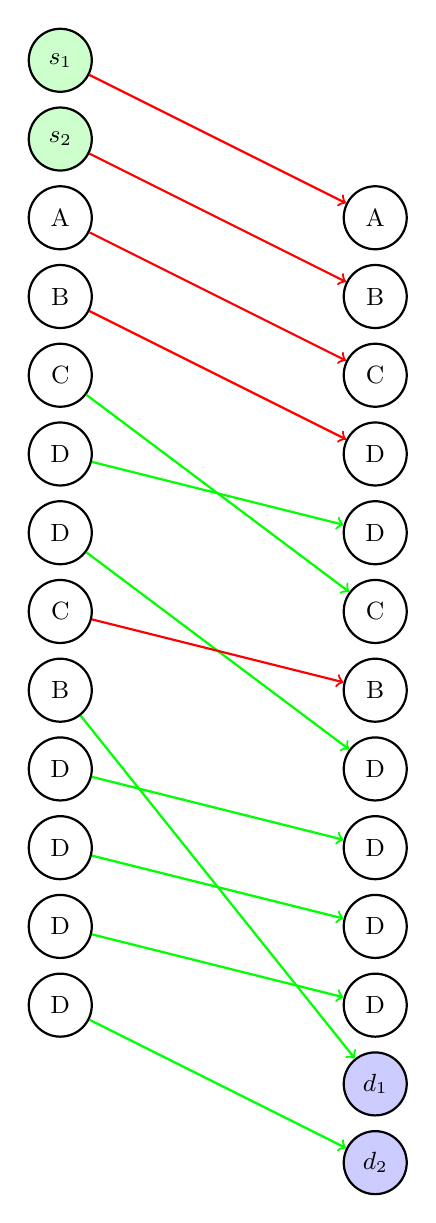
\begin{tikzpicture}[node distance={10mm}, thick, auto=center, main/.style = {draw, circle}]
                \tikzstyle{main} = [circle, draw, minimum size=0.8cm, font=\small]
                \tikzstyle{source} = [circle, draw, minimum size=0.8cm, font=\small, fill=green!20]
                \tikzstyle{dest} = [circle, draw, minimum size=0.8cm, font=\small, fill=blue!20]

                % Source nodes (left column, green background)
                \node[source] (s1) {$s_1$};
                \node[source] (s2) [below of=s1] {$s_2$};
                
                % Tree nodes (left column, red border)
                \node[main] (t1) [below of=s2] {A};
                \node[main] (t2) [below of=t1] {B};
                \node[main] (t3) [below of=t2] {C};
                \node[main] (t4) [below of=t3] {D};
                \node[main] (t5) [below of=t4] {D};
                \node[main] (t6) [below of=t5] {C};
                \node[main] (t7) [below of=t6] {B};
                \node[main] (t8) [below of=t7] {D};
                \node[main] (t9) [below of=t8] {D};
                \node[main] (t10) [below of=t9] {D};
                \node[main] (t11) [below of=t10] {D};
                
                % Tree nodes (right column, red border)
                \node[main] (r1) [right of=t1, xshift=3cm] {A};
                \node[main] (r2) [below of=r1] {B};
                \node[main] (r3) [below of=r2] {C};
                \node[main] (r4) [below of=r3] {D};
                \node[main] (r5) [below of=r4] {D};
                \node[main] (r6) [below of=r5] {C};
                \node[main] (r7) [below of=r6] {B};
                \node[main] (r8) [below of=r7] {D};
                \node[main] (r9) [below of=r8] {D};
                \node[main] (r10) [below of=r9] {D};
                \node[main] (r11) [below of=r10] {D};
                
                % Destination nodes (right column, blue background)
                \node[dest] (d1) [below of=r11] {$d_1$};
                \node[dest] (d2) [below of=d1] {$d_2$};
                
                \draw[red, ->] (s1) -- (r1);
                \draw[red, ->] (s2) -- (r2);
                \draw[red, ->] (t1) -- (r3);
                \draw[red, ->] (t2) -- (r4);
                \draw[green, ->] (t3) -- (r6);
                \draw[green, ->] (t4) -- (r5);
                \draw[green, ->] (t5) -- (r8);
                \draw[red, ->] (t6) -- (r7);
                \draw[green, ->] (t7) -- (d1);
                \draw[green, ->] (t8) -- (r9);
                \draw[green, ->] (t9) -- (r10);
                \draw[green, ->] (t10) -- (r11);
                \draw[green, ->] (t11) -- (d2);
            \end{tikzpicture} 
        \caption[Reduction full example]{Example of an optimal perfect matching for the graph $G$ of the MWPBM instance $r((S = ABCDDCBDDDD, p = 2))$. Green edges weigh $0$, while red edges weigh $1$.}
        \label{fig:reduction_example}
    \end{figure}
\end{example}